\documentclass[dvipdfmx]{jarticle}
\pagestyle{empty}
\usepackage{tikz}
\usetikzlibrary{calc,shapes,arrows.meta,decorations.pathmorphing}
\newcommand{\ttx}{\texttt{x}}
\newcommand{\tteq}{\texttt{=}}
\begin{document}
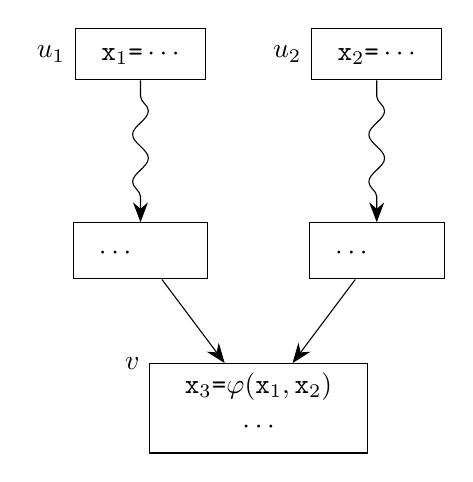
\begin{tikzpicture}
    \node[draw,label={180:{$u_1$}}] (U1) at (-1.5,4.5) {\begin{tabular}{l}
            $\ttx_1\tteq\cdots$
        \end{tabular}};
    \node[draw,label={180:{$u_2$}}] (U2) at (1.5,4.5) {\begin{tabular}{l}
            $\ttx_2\tteq\cdots$
        \end{tabular}};
    \node[draw] (U11) at (-1.5,2) {\begin{tabular}{c}
            \vbox to 10pt{\vfill\hbox to 30pt{$\cdots$}}
        \end{tabular}};
    \node[draw] (U21) at (1.5,2) {\begin{tabular}{c}
            \vbox to 10pt{\vfill\hbox to 30pt{$\cdots$}}
        \end{tabular}};
    \node[draw,label={165:{$v$}}] (V0) at (0,0) {\begin{tabular}{c}
            \vbox to 10pt{\hbox to 60pt{\hfill$\ttx_3\tteq\varphi(\ttx_1,\ttx_2)$\hfill}\vfill} \\
            $\cdots$
        \end{tabular}};
    \draw[-{Stealth[scale=1.5]},
        decorate,
        decoration={
                snake, amplitude=1mm,
                segment length=6mm,
                pre length=2mm,
                post length=3mm
            }
    ] (U1) -- (U11);
    \draw[-{Stealth[scale=1.5]},
        decorate,
        decoration={
                snake, amplitude=1mm,
                segment length=6mm,
                pre length=2mm,
                post length=3mm
            }
    ] (U2) -- (U21);
    \path[-{Stealth[scale=1.5]}] (U11) edge (V0) (U21) edge (V0);
\end{tikzpicture}
\end{document}